% Report
\documentclass{article}

% Here set the various packages
% Packages to load
\usepackage[english]{babel}
% %%% Support some german text
% \usepackage{ngerman}
% \usepackage[latin1]{inputenc}   % für Umlaute
%%%
% \usepackage[utf8]{inputenc}
\usepackage[T1]{fontenc}
\usepackage{microtype}

%%%
% \usepackage[inline]{enumitem} % Required for the "description" list.

%%% Fix for not hyperlinking citations
\makeatletter
\let\NAT@parse\undefined
\makeatother
\usepackage{hyperref}
% 
\usepackage{cite}
% \ifx\pdfoutput\undefined
% 	\usepackage{graphicx}
% \else
% 	\usepackage[pdftex]{graphicx}
% \fi
\usepackage{graphicx}
\graphicspath{{Figures/}}
\usepackage{amsmath}
% \interdisplaylinepenalty=2500

% Shading of questions. Use the "shaded" environment or the "\hl{}" command.
\usepackage{framed}
% \usepackage[dvipsnames]{color}
\usepackage[svgnames]{xcolor}
\usepackage{soul}
% Nice colours: Gainsboro, LightGoldenrod, LightSteelBlue
% furter ref: https://www.latextemplates.com/svgnames-colors
\definecolor{shadecolor}{named}{Gainsboro}
\sethlcolor{Gainsboro}

%%% Todo margin notes (enable/disable)
\usepackage{todonotes}
% \usepackage[disable]{todonotes}
%%%

%eof



%%%

\title{Programming of Supercomputers\\Worksheet 1}
\author{Oleksandr Voloshyn\\ Qunsheng Huang\\ Tommaso Bianucci}
\date{\today}

\begin{document}

\maketitle
\renewcommand{\abstractname}{Group members's contributions}
\begin{abstract}
	% Here write the contributions of the members of the group
	Oleksandr Voloshyn: Worked on 4.1, 4.2, 4.3

	Tommaso Bianucci: Worked on 4.1, 4.2, 4.3
	
	Qunsheng Huang: Worked on 4.1, 4.3, 4.4
\end{abstract}

\section{Performance baseline} % Name of assignment 1
\subsection{GNU Profiler} % Name of sub-assignment
% \subsubsection{Questions}
\begin{enumerate}
\item{Which routines took 80\% or more of the execution time of the benchmark?
}
\begin{enumerate}
	\item{Serial}
	\begin{itemize}
		\item{EvalEOSForElems(Domain\&, double*, int, int*, int) --- 28.18\%}
		\item{CalcHourglassControlForElems(Domain\&, double*, double) --- 17.10\%}
		\item{CalcFBHourglassForceForElems(...) --- 15.76\%}
		\item{CalcKinematicsForElems(Domain\&, double, int) --- 11.84\%}
		\item{IntegrateStressForElems(Domain\&, double*, double*, double*, double*, int, int) --- 10.98\%}
\\\\These functions account for 83.86\% of total execution time
	\end{itemize}
	\item{OpenMP}
	\begin{itemize}
		\item{CalcHourglassControlForElems(Domain\&, double*, double) --- 29.90\%}
		\item{ApplyMaterialPropertiesForElems(Domain\&) --- 22.58\%}
		\item{CalcFBHourglassForceForElems(...) --- 15.84\%}
		\item{IntegrateStressForElems(...) --- 14.28\% }
\\\\These functions account for 82.60\% of total execution time
	\end{itemize}
	\item{MPI}
	\begin{itemize}
		\item{EvalEOSForElems(Domain\&, double*, int, int*, int) --- 24.44\%}
		\item{LagrangeNodal(Domain\&) --- 21.86\%}
		\item{CalcFBHourglassForceForElems(..) --- 16.67\%}
		\item{CalcKinematicsForElems(Domain\&, double, int) --- 11.12\%}
		\item{IntegrateStressForElems(...) --- 10.15\%}
\\\\These functions account for 84.24\% of total execution time
	\end{itemize}
	\item{Hybrid}
	\begin{itemize}
		\item{CalcFBHourglassForceForElems(..) --- 23.05\%}											\item{EvalEOSForElems(Domain\&, double*, int, int*, int) --- 21.22\%}
		\item{LagrangeNodal(Domain\&) --- 18.95\%}
		\item{IntegrateStressForElems(...) --- 13.02\%}
		\item{CalcKinematicsForElems(Domain\&, double, int) --- 10.29\%}
\\\\These functions account for 86.53\% of total execution time
	\end{itemize}
\end{enumerate}
\item{Is the measured execution time of the application affected by gprof? Hint: use the time command to determine this.}\\\\
The measured execution time does not differ with use of gprof. This was tested with the four benchmarks with the following results:
\begin{center}
\begin{tabular}{|c|c|c|}
\hline
&Time without Gprof (s) & Time with Gprof (s)\\
\hline
Serial &53.90&53.88\\ \hline
OpenMP &21.06&20.95\\ \hline
MPI &120.78&120.84\\ \hline
Hybrid &46.9&45.95\\ \hline
\end{tabular}
\end{center}
Each benchmark was run 2-3 times with and without gprof. The times did vary slightly but indicated that the usage of gprof did not change th execution time. The results in the above table can be seen in the attached gprof files.
\item{Can gprof analyze the loops (for, while, do-while, etc.) of the application?}\\\\
No, gprof cannot be used to analyse loops.
\item{Is gprof capable of analyzing parallel applications?}\\\\
Yes, gprof can be used to analyze some parallel applications. However, typically only the performance of the main thread is recorded (as in the case of MPI implementations). The obscuring of information can be seen especially in the case of openMP, where the code spends more than 50\% of the time in "frame dummy", a function that does not exist in source code.
\item{What is necessary to analyze parallel applications?}\\\\
Gprof typically only produces one gmon.out output file for the main process. However, in a parallel process, multiple output files are required. When using MPI processes, it is possible to inform gprof, via environmental variables, of the number of threads produced and run. One gmon.out is then produced per thread. These files can then be aggregated to determine the overall behavior of all threads together or analyzed separately.
\item{Where there performance differences between the GNU++ and the Intel compiler?}\\\\
There were differences between the two compilers. In general, the code compiled by the Intel compiler was slightly faster. The difference between the code compiled by the two compilers is approximately 2s and this varied slightly each job. Four jobs were run using the automated script in Section 4.2 of the assignment - in both cases, the Intel compiled code ran approximately ~2s faster with the optimal.
\end{enumerate}

\subsection{Compiler flags}
\begin{enumerate}
\item{Look at the compilers help (by issuing icc -help and gcc -help). How many opti-
mization flags are available for each compiler (approximately)?}\\\\
gcc-help shows approximately 100 compiler flags, icpc-help show approximately 18 optimization flags, 8 interprocedural optimization flags, 60 advanced optimization options and 20 profile guided optimizations, for a total of 106 flags.
\item{Given how much time it takes to evaluate a combination of compiler flags, is it realistic to test all possible combinations of available compiler flags? What could be a possible solution?}\\\\
 Each test run takes approximately 40-50 seconds to complete, excluding the time required for compilation of the code. Given that there are more than 100 optimiation flags for each compiler, we can conservatively estimate that the total time to completion would exceed $6\times10^{32}s$, which is completely unfeasible. Instead, it would make sense for us to examine the code to determine what possible bottlenecks exist and apply flags that could improve the situation. 
\item{Which compiler and optimization flags combination produced the fastest binary?}\\\\
For the GNU++ compiler, we determined that the effect of the flags was somewhat inconsistent. We performed a simple statistical analysis of the effects of the flags over 3 runs. Overall, we observed that the flags "-march=native" and "-funroll-loops" were constantly associated with binaries with the best performance.

For the Intel compiler, the fastest binary only used "-unroll" flag with a time of 50.43s to completion with a speedup of 1.00258. The second fastest binary was without flags with a time of 50.56.

The fastest binary from both compilers was compiled using the Intel compiler with the "-unroll" flag.
\end{enumerate}

\subsection{Optimization pragmas}
\begin{enumerate}
\item{What is the difference between Intels simd, vector and ivdep \#pragma directives?}\\\\
The three pragmas allow the compiler to ignore certain requirements when vectorizing. The simd pragma forces vectorization to occur, ignoring safety or cost. The vector pragma forces the compiler to ignore cost when deciding to vectorize (as a result the code may run slower after vectorization). The ivdep pragma instructs compiler to ignore assumed vector dependencies - ie compiler may choose to treat assumed dependencies as proven dependencies. This pragma instructs compiler to ignore such assumptions and proceed with vectorisation.
\item{Why did you choose to apply the selected #pragma in the particular location?}\\\\
We chose to apply \verb!#pragma loop_count avg(27000)! to the function \verb!CalcHourglassControlForElems! in lulesh.cc. When running the task in serial, more than 70\% of overall runtime time was spent in this function. This function contains a highly complicated loop that may require specific treatment for optimization.
\end{enumerate}

\subsection{Inline assembler}
\begin{enumerate}
\item{Is the inline assembler necessarily faster than compiler generated code?}\\\\
Not necessarily. The speed increase is dependent on the implementation on the code - especially when modern compilers already implement many forms of optimization. It is often likely that hand-written assembler code is often slower than compiler optimized assembler code. However, there do exist specific cases where an inline assembler may be faster. The most relevant cases to this module include:
\begin{itemize}
\item{Implement instructions which are not yet possible in the current language. For example, certain operations, such as a full-multiplication operator in C---2N-bit result from N-bit inputs. Most x86 CPUs can, however, perform this operation in a single instruction. In these rare cases, it would be beneficial to use optimal functions that belong to the specific CPU when available.}
\item{Spot-optimizing specific lines of code. For example, compilers may not optimally vectorize complicated loops, since it has to deal with many general cases. If the programmer understands the problem well, it may be beneficial to use the inline assembler to perform the loop operations.}
\end{itemize}
\item{On the release of a CPU with new instructions, can you use an inline assembler to take advantage of these instructions if the compiler does not support them yet?}\\\\
Yes. One benefit to inline assemblers is that it allows access to processor specific instructions which the compiler may not support. Examples may include FPU instructions that may be faster than compiler generated floating operations. However, the onus of correct usage of these commands then falls on the programmer.
\item{What is AVX-512? Which CPUs support it? Is there any compiler or language support for these instructions at this moment?}\\\\
AVX stands for Advanced Vector Extensions SIMD instructions. AVX-512 are the 512-bit extensions to the preexisting AVX/AVX2 instructions. They were first supported by the Xeon-Phi x200 (Knights Landing) and Skylake-X CPUs. Note that AVX-512 is not the first 512-bit SIMD instructions released by Intel. These commands are supported in the intel C++ compiler under the namespace AVX. The -xCOMMON-AVX512 flag can be used for auto-vectorization using AVX-512 functions.

\end{enumerate}

% Figure example
%\begin{figure}[h!] % h=here, t=top, b=bottom, p=(extra)page, !=force
 %	\begin{center}
 %		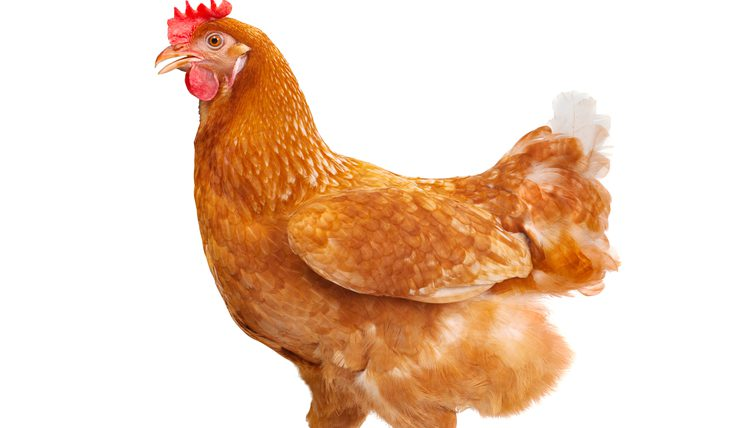
\includegraphics[width=.9\linewidth]{figure.png} % It searches in the Figures/ folder!
 %		\caption{Caption text}
 %		\label{fig:figureLabelName}
 %	\end{center}
%\end{figure}

\section{Name of assignment 2}
\subsection{Name of sub-assignment 2.1}
Lorem ipsum

\end{document}

%eof
